\documentclass[12pt,letterpaper,sans]{moderncv}

\moderncvstyle{banking}
\moderncvcolor{blue}
\renewcommand{\familydefault}{\sfdefault}

\usepackage[utf8]{inputenc}

\usepackage[leftmargin=22pt]{etaremune}
\usepackage{lipsum}
\usepackage[margin = 1in]{geometry}
\usepackage[none]{hyphenat}


\newcommand*{\paper}[4]{\textit{#1}\newline #2. \newline\href{#3}{\textcolor{blue}{#4}}}
\newcommand*{\blink}[2]{\textit{\href{#1}{\textcolor{blue}{#2}}}}

\fancyfoot[L]{\textcolor{gray}{\today}}

\firstname{Eric J.}
\familyname{Meier, Ph.D.\vspace*{12pt}}
%\title{CV}
%\born{July 21, 1991}
\address{Scientist $\bullet$ Quantum Group $\bullet$ Materials Physics and Applications Division}{Los Alamos National Laboratory $\bullet$ Los Alamos, NM 87545}
%\mobile{(000) 111 1111}
\phone{(505) 665-6537}
%\fax{(000) 111 1113}
\email{ejmeier@lanl.gov}
\homepage{ericjmeier.com}
%\extrainfo{2510 A S Vine St. Urbana, IL 61801}
% \photo[70pt][0.4pt]{./assets/imgs/photo_Meier_Eric.jpg}
%\quote{"A witty and playful quotation" - John Smith}
\patchcmd{\makehead}% <cmd>
  {\\[2.5em]}% <search>
  {\hfill\raisebox{-1.4cm}[0pt][0pt]{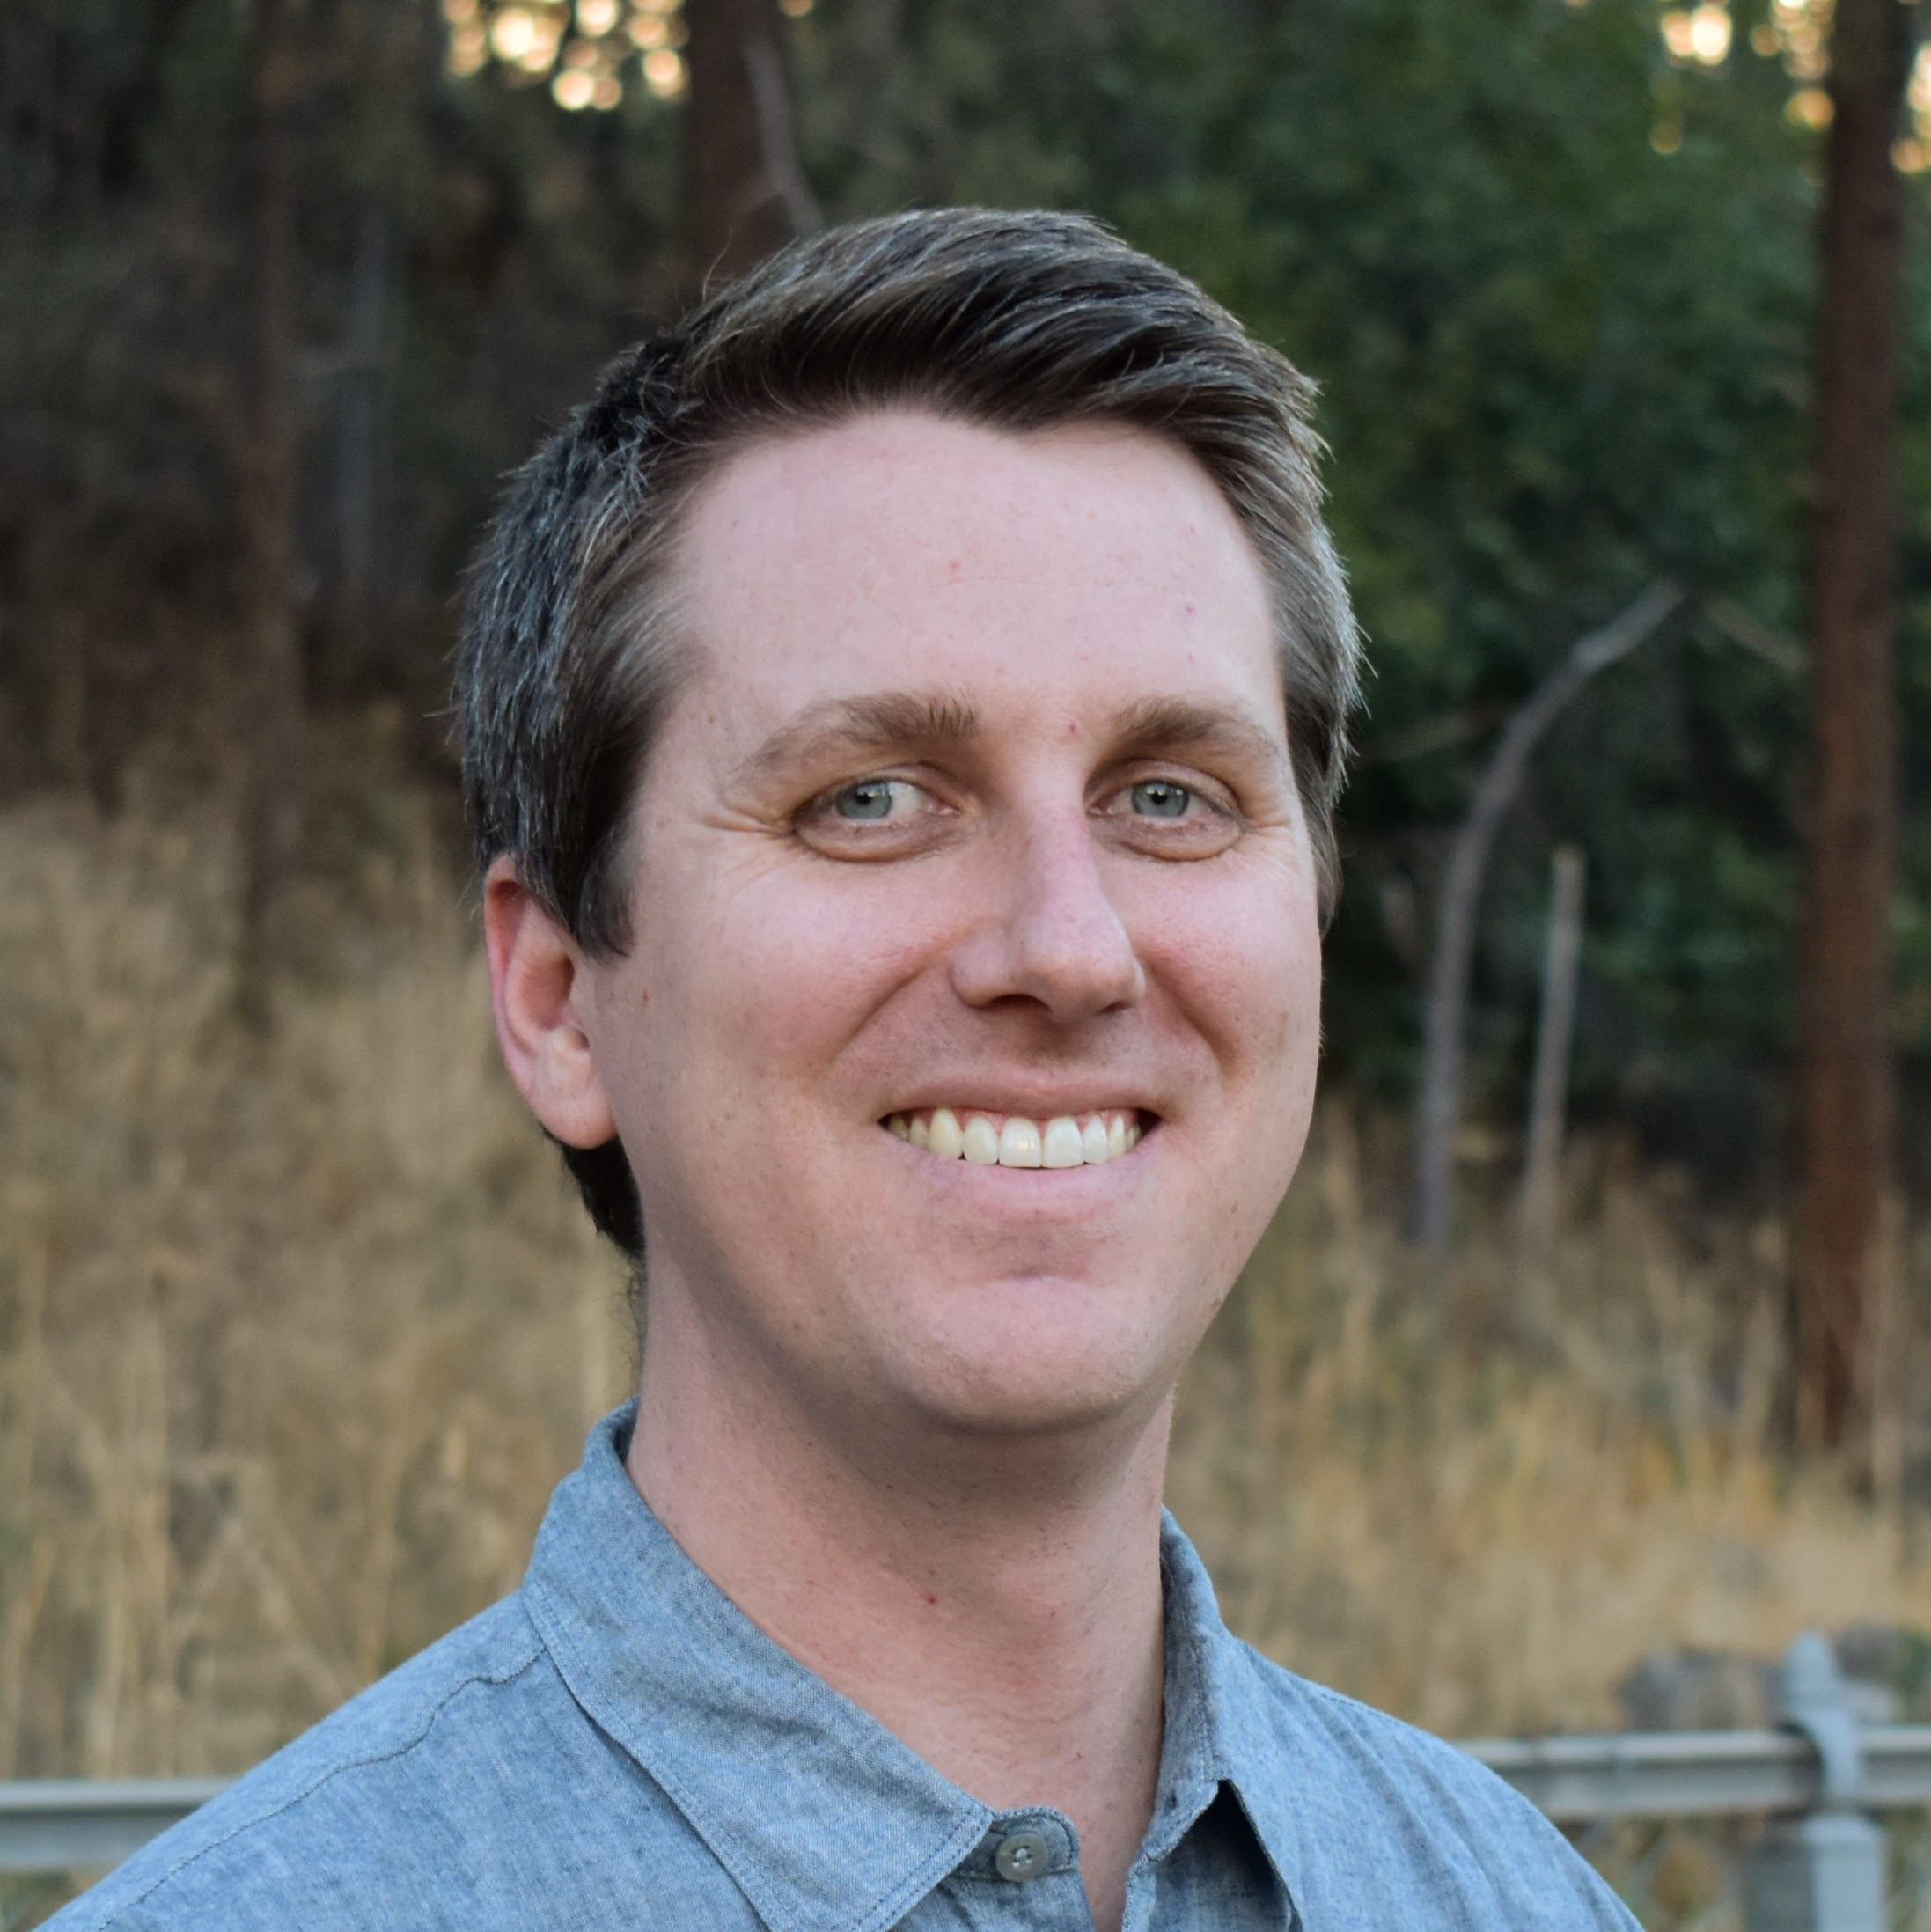
\includegraphics[width=.18\textwidth]{./assets/imgs/photo_Meier_Eric.jpg}}\\[2.5em]}% <replace>
  {}{}% <success><failure>
%----------------------------------------------------------------------------------------

\begin{document}


%----------------------------------------------------------------------------------------
%	CURRICULUM VITAE - LAST UPDATED 5/10/2023
%----------------------------------------------------------------------------------------

\makecvtitle % Print the CV title

%----------------------------------------------------------------------------------------
%	EDUCATION SECTION
%----------------------------------------------------------------------------------------

\section{Education}

\cventry{}{\textnormal{The University of Illinois at Urbana-Champaign}}{Ph.D. physics}{2019}{}{Thesis: \blink{https://uofi.box.com/shared/static/9mzcm685c37wictkydgacejmtyhsgdg8.pdf}{Momentum-Space Lattices for Ultracold Atoms}, Advisor: Bryce Gadway}  % Arguments not required can be left empty
\cventry{}{\textnormal{Denison University. Granville, Ohio}}{B.S. physics, cum laude}{2014}{}{Thesis: \blink{https://uofi.box.com/shared/static/cu7je3u8vpb84vf9httucgxk4whbgk1x.pdf}{Statistical Modeling of Jets in Active Galactic Nuclei}, Advisor: Dan Homan}

%----------------------------------------------------------------------------------------
%	WORK EXPERIENCE SECTION
%----------------------------------------------------------------------------------------

\section{Research}

\subsection{Professional}

\cventry{}{\textnormal{Los Alamos National Laboratory}}{Scientist, Quantum Group, MPA}{2023--Present}{}{I work on a myriad of projects in quantum information science using experimental atomic physics.}

\subsection{Postdoctoral}

\cventry{}{\textnormal{Los Alamos National Laboratory}}{Director's Postdoctoral Fellow, MPA--Q}{2021--2023}{}{I primarily worked toward building apparatuses for quantum computing and sensing with ultracold rubidium and strontium atoms.}

\cventry{}{\textnormal{The University of Illinois at Urbana-Champaign}}{Postdoctoral Research Associate, Gadway/DeMarco Lab}{2019--2021}{}{I worked with three different teams in the lab. (1) My primary role was the construction of a ground state sodium-rubidium molecule apparatus for use in quantum information experiments. (2) I built a system that uses potassium Rydberg atoms trapped in optical tweezers for analog quantum simulation experiments. (3) I helped in a mentorship role on the Bose--Einstein condensate apparatus I constructed as part of my graduate work.}

\subsection{Graduate}

\cventry{}{\textnormal{The University of Illinois at Urbana-Champaign}}{Research Assistant, Advisor: Bryce Gadway}{2014--2019}{}{As the first graduate student in the Gadway Lab, I built and operated a rubidium Bose--Einstein condensate apparatus that engineered synthetic lattices of atomic momentum-states for the analog quantum simulation of condensed matter phenomena.}

%------------------------------------------------

\subsection{Undergraduate}

\cventry{}{\textnormal{Denison University. Granville, Ohio}}{Researcher, Advisor: Steven Olmschenk}{2014}{}{I worked toward building a trapped ion quantum computing system using lanthanum ions.}

\cventry{}{\textnormal{Denison University. Granville, Ohio}}{Researcher, Advisor: Dan Homan}{2012--2014}{}{I wrote computer simulations of relativistic extragalactic jets in an effort to match typical observed acceleration profiles found in the MOJAVE program database.}

%----------------------------------------------------------------------------------------
%	Skills
%----------------------------------------------------------------------------------------

\section{Skills}
\subsection{Experimental Physics Skills}
Laser Operation, Alignment, \& Locking $\bullet$ Vacuum Chamber Assembly \& Baking $\bullet$ Laser Safety Interlock Design and Implementation $\bullet$ Experimental Optimization with Machine Learning $\bullet$ Electromagnet Design \& Control (including high-fields for Feshbach Resonances) $\bullet$ Optical Fibers/Fiber Coupling/Fiber Splicing $\bullet$ Data Analysis $\bullet$ Computer Simulation $\bullet$ Basic Electronics Design $\bullet$ Surface-Mount and Through-Hole Soldering $\bullet$ Atomic Spectroscopy Techniques (Saturated Absorption, Polarization, Modulation Transfer) $\bullet$ Resonant Atomic Imaging $\bullet$ 2D and 3D Magneto-Optical Trapping $\bullet$ Optical Pumping $\bullet$ Optical Molasses $\bullet$ Optical Dipole Trapping \& Evaporation $\bullet$ Bose--Einstein Condensation $\bullet$ Two-Species Mixtures $\bullet$ Light-Induced Atomic Desorption $\bullet$ Digital Micromirror Devices \& Spatial Light Modulators $\bullet$ Active Optical Elements (Tapered Amplifiers, Acousto- and Electro-Optic Modulators, Shutters, Raman Fiber Amplifiers) $\bullet$ Radio-Frequency Source Design and Implementation $\bullet$ Optical Cavity Laser Locking $\bullet$ Basic Woodworking \& Machining

\subsection{Computer Skills \& Languages}
Adobe Photoshop \& Illustrator $\bullet$ Wolfram Mathematica $\bullet$ Matlab $\bullet$ Python $\bullet$ LabVIEW \& LabVIEW FPGA $\bullet$ 3D Modeling and Design in Solidworks $\bullet$ Andor Basic $\bullet$ Microsoft Office $\bullet$ Computer Assembly $\bullet$ \LaTeX $\bullet$ American Sign Language (beginner)

\subsection{Soft Skills}
Flexibility $\bullet$ Effective and Clear Communication $\bullet$ Attention to Detail $\bullet$ Teamwork \& Cooperation $\bullet$ Time Management $\bullet$ Internal Motivation




%----------------------------------------------------------------------------------------
%	Publications
%----------------------------------------------------------------------------------------

\section{Publications}

\subsection{Selected}

\begin{etaremune}[start=13,topsep=0pt,itemsep=4pt,partopsep=0pt,parsep=0pt]

\item \paper{Observation of the topological Anderson insulator in disordered atomic wires}{\textbf{Eric.~J. Meier}, Fangzhao Alex An, Alexandre~Dauphin, Maria Maffei, Pietro Massignan, Taylor L.\ Hughes, and Bryce Gadway}{http://science.sciencemag.org/content/362/6417/929.full?ijkey=bU33NGPrjqfmg&keytype=ref&siteid=sci}{Science \textbf{362}, 6417 (2018)}
\begin{itemize}
\item selected for a \href{https://www.nature.com/articles/s41567-018-0399-y}{\textcolor{blue}{research highlight in Nature Physics}}
\end{itemize}

\item \paper{Observation of the topological soliton state in the Su-Schrieffer-Heeger model}{\textbf{Eric J.\ Meier}, Fangzhao Alex An, and Bryce Gadway}{http://www.nature.com/articles/ncomms13986}{Nature Communications \textbf{7}, 13986 (2016)}

\item \paper{Atom-optics simulator of lattice transport phenomena}{\textbf{Eric J.\ Meier}, Fangzhao Alex An, and Bryce Gadway}{http://journals.aps.org/pra/abstract/10.1103/PhysRevA.93.051602}{Physical Review A \textbf{93}, 051602(R) (2016)}
\end{etaremune}

\subsection{Other}

\begin{etaremune}[topsep=0pt,itemsep=4pt,partopsep=0pt,parsep=0pt]

\item \paper{Qudit entanglers using quantum optimal control}{Sivaprasad~Omanakuttan, Anupam~Mitra, \textbf{Eric~J.~Meier}, Michael~J.~Martin, Ivan~H.~Deutsch}{https://journals.aps.org/prxquantum/abstract/10.1103/PRXQuantum.4.040333}{PRX Quantum 4, 040333 (2023)}

\item \paper{Nonlinear Dynamics in a Synthetic Momentum-State Lattice}{Fangzhao~Alex~An, Bhuvanesh~Sundar, Junpeng~Hou, Xi-Wang~Luo, \textbf{Eric~J.~Meier}, Chuanwei~Zhang, Kaden~R.~A.~Hazzard, and Bryce~Gadway}{https://journals.aps.org/prl/abstract/10.1103/PhysRevLett.127.130401}{Physical Review Letters \textbf{127}, 130401 (2021)}
\begin{itemize}
\item selected as \emph{Editor's Suggestion}
\end{itemize}

\item \paper{Interactions and Mobility Edges: Observing the Generalized Aubry-Andr{\'e} Model}{Fangzhao~Alex~An, Karmela~Padavi{\'c}, \textbf{Eric~J.~Meier}, Suraj~Hegde, Sriram~Ganeshan, J.~H.~Pixley, Smitha~Vishveshwara, and Bryce~Gadway}{https://journals.aps.org/prl/abstract/10.1103/PhysRevLett.126.040603}{Physical Review Letters \textbf{126}, 040603 (2021)}
\begin{itemize}
\item selected as \emph{Editor's Suggestion}
\end{itemize}

\item \paper{Nondestructive dispersive imaging of rotationally excited ultracold molecules}{Qingze Guan, Michael Highman, \textbf{Eric~J.~Meier}, Garrett~R.~Williams, Vito~Scarola, Brian~DeMarco, Svetlana~Kotochigova, and Bryce~Gadway}{http://dx.doi.org/10.1039/D0CP03419C}{Physical Chemistry Chemical Physics \textbf{22}, 20531 (2020)}

\item \paper{Counterdiabatic control of transport in a synthetic tight-binding lattice}{\textbf{Eric J.\ Meier}, Kinfung Ngan, Dries Sels, and Bryce Gadway}{https://journals.aps.org/prresearch/abstract/10.1103/PhysRevResearch.2.043201}{Physical Review Research \textbf{2}, 043201 (2020)}
\begin{itemize}
\item selected as \emph{Editor's Suggestion}
\end{itemize}

\item \paper{Exploring quantum signatures of chaos on a Floquet synthetic lattice}{\textbf{Eric J.\ Meier$^*$}, Jackson Ang’ong’a$^*$, Fangzhao Alex An, and Bryce Gadway}{https://journals.aps.org/pra/abstract/10.1103/PhysRevA.100.013623}{Physical Review A \textbf{100}, 013623 (2019)}
\begin{itemize}
\item selected as \emph{Editor's Suggestion}
\end{itemize}

\item \paper{Engineering a flux-dependent mobility edge in disordered zigzag chains}{Fangzhao Alex An, \textbf{Eric J.\ Meier}, and Bryce Gadway}{https://journals.aps.org/prx/abstract/10.1103/PhysRevX.8.031045}{Physical Review X \textbf{8}, 031045 (2018)}

\item \paper{Correlated dynamics in a synthetic lattice of momentum states}{Fangzhao Alex An, \textbf{Eric J.\ Meier}, Jackson Ang'ong'a, and Bryce Gadway}{https://link.aps.org/doi/10.1103/PhysRevLett.120.040407}{Physical Review Letters \textbf{120}, 040407 (2018)}

\item \paper{Diffusive and arrested transport of atoms under tailored disorder}{Fangzhao Alex An, \textbf{Eric J.\ Meier}, and Bryce Gadway}{https://www.nature.com/articles/s41467-017-00387-w}{Nature Communications \textbf{8}, 325 (2017)}

\item \paper{Direct observation of chiral currents and magnetic reflection in atomic flux lattices}{Fangzhao Alex An, \textbf{Eric J.\ Meier}, and Bryce Gadway}{http://advances.sciencemag.org/content/3/4/e1602685}{Science Advances \textbf{3}, e1602685 (2017)}

\end{etaremune}

%----------------------------------------------------------------------------------------
%	Presentations
%----------------------------------------------------------------------------------------

\section{Presentations}

\subsection{Oral Presentations}

\begin{etaremune}[topsep=0pt,itemsep=4pt,partopsep=0pt,parsep=0pt]

\item Air Force Research Lab and Sandia Technical Exchange Seminar (invited)
\newline
\emph{Neutral Atom Quantum Information Science}
\newline
July 2023 virtual

\item BEC2018X (invited)
\newline 
\blink{http://thetis.ph.tsukuba.ac.jp/~hatsugai/modules/pico4/workshop2018x/meie.pdf}{Quantum simulation of one-dimensional topological insulators with cold atoms}
\newline 
December 2018 at the University of Tsukuba in Tokyo, Japan

\item Midwest Cold Atom Workshop 2017 (invited)
\newline 
\emph{Correlated phenomena in synthetic momentum-space lattices}
\newline 
November 2017 at the University of Michigan in Ann Arbor, Michigan

\item DAMOP 2019, Session: ``Dynamics of Cold Atoms in Optical Lattices''
\newline 
\emph{Fast eigenstate preparation in a synthetic lattice by counter-diabatic driving}
\newline 
May 2019 in Milwaukee, Wisconsin

\item DAMOP 2017, Session: ``New Topological Quantum Matter''
\newline 
\emph{Disordered topological wires in a momentum-space lattice}
\newline 
June 2017 in Sacramento, California

\item DAMOP 2016, Session: ``Progress in Spin-Orbit Coupling''
\newline 
\emph{Direct observation of edge states in the Su--Schrieffer--Heeger model with bosonic atoms in a momentum space lattice}
\newline 
May 2016 in Providence, Rhode Island

\end{etaremune}

\subsection{Posters}

\begin{etaremune}[topsep=0pt,itemsep=4pt,partopsep=0pt,parsep=0pt]

\item DAMOP 2023
\newline
\emph{Experimental progress towards quantum control of strontium qudits}
\newline
June 2023 at in Spokane, Washington

\item Midwest Cold Atom Workshop 2019
\newline
\emph{Evidence for the topological Anderson insulator}
\newline
November 2019 at Northwestern University in Evanston, Illinois

\item International Conference on Atomic Physics 2018
\newline
\emph{Evidence for the topological Anderson insulator}
\newline
July 2018 in Barcelona, Spain

\item Midwest Cold Atom Workshop 2017
\newline
\emph{Disordered topological wires}
\newline
November 2017 at the University of Michigan in Ann Arbor, Michigan

\item DAMOP 2017
\newline
\emph{Disordered wires and quantum chaos in a momentum-space lattice}
\newline
June 2017 in Sacramento, California

\item Midwest Cold Atom Workshop 2016
\newline
\emph{Quantum simulation of topological wires}
\newline
October 2016 at the University of Chicago in Chicago, Illinois

\item DAMOP 2016
\newline
\emph{Atom optics simulator of lattice transport phenomena}
\newline
May 2016 in Providence, Rhode Island

\item Midwest Cold Atom Workshop 2015
\newline
\emph{Towards studying topological matter with cold atoms in optical lattices}
\newline
November 2015 at the University of Wisconsin at Madison

\end{etaremune}

%----------------------------------------------------------------------------------------
%	AWARDS SECTION
%----------------------------------------------------------------------------------------

\section{Honors and Awards}

\cvitem{2021}{Director's Postdoctoral Fellow, Los Alamos National Laboratory
\small{
\begin{itemize}
\item based on academic and research accomplishments, the strength of the proposed research, as well as their potential impact at the Laboratory
\end{itemize}}}

\cvitem{2018}{Drickamer Research Fellowship, University of Illinois at Urbana-Champaign
\small{
\begin{itemize}
\item a graduate fellowship awarded to a student who has demonstrated significant ability in research
\end{itemize}}}

\cvitem{2016}{Scott Anderson Award, University of Illinois at Urbana-Champaign
\small{
\begin{itemize}
\item recognizes the year's outstanding physics graduate teaching or research assistants
\end{itemize}}}

\cvitem{2014}{Samuel C. Wheeler Award for Excellence in Physics, Denison University
\small{
\begin{itemize}
\item excellence in the understanding and doing of physics combined with leadership in the department
\end{itemize}}}

\cvitem{2012, 2013}{Physics Department Fellow, Denison University}

\cvitem{2012}{Inducted, Sigma Pi Sigma National Physics Honor Society}

\cvitem{2012, 2013}{Anderson Summer Research Assistantship Award, Denison University
\small{
\begin{itemize}
\item funding for summer-term research awarded to excellent proposals in all fields of science
\end{itemize}}}

\cvitem{2012}{Ron Winters Emeritus Faculty Scholar Award, Denison University
\small{
\begin{itemize}
\item outstanding undergraduate physics research
\end{itemize}}}

\cvitem{2011}{Excellence in Introductory Physics Award, Denison University}

\cvitem{2009}{Boy Scouts of America Eagle Scout Award. Troop 11, Kingsville, Ohio}

%----------------------------------------------------------------------------------------
%	Teaching
%----------------------------------------------------------------------------------------

\section{Teaching}

\subsection{Graduate}

\cventry{}{\textnormal{The University of Illinois at Urbana-Champaign}}{Teaching Assistant, College Physics: E\&M \& Modern}{2018, 2019}{}{I taught small class sections (30 students) in this second introductory physics course for non-majors.
\begin{itemize}
\item Ranked `Excellent Teacher' based on student evaluations
\end{itemize}
}

\cventry{}{\textnormal{The University of Illinois at Urbana-Champaign}}{Teaching Assistant, Introductory Mechanics}{2014}{}{I taught small class sections (30 students) in this introductory physics course for physics majors.
\begin{itemize}
\item Ranked `Excellent Teacher' based on student evaluations
\end{itemize}
}

\subsection{Undergraduate}

\cventry{}{\textnormal{Denison University. Granville, Ohio}}{Laboratory Teaching Assistant, Introductory Astronomy}{2013--2014}{}{In addition to teaching students how to use reflecting and refracting telescopes and aiding them in their observations, I was in charge of telescope assembly, disassembly, and storage.}

\cventry{}{\textnormal{Denison University. Granville, Ohio}}{Laboratory Teaching Assistant, Introductory Physics}{2012--2014}{}{Working in conjunction with the course's professor, I facilitated students in performing their experiments.}

\cventry{}{\textnormal{Denison University. Granville, Ohio}}{University Tutor}{2011--2014}{}{%I was employed by the University to tutor students on both a walk-in and a by-appointment basis in introductory physics and chemistry.
}


\end{document}















